% *======================================================================*
%  Cactus Thorn template for ThornGuide documentation
%  Author: Ian Kelley
%  Date: Sun Jun 02, 2002
%  $Header$
%
%  Thorn documentation in the latex file doc/documentation.tex
%  will be included in ThornGuides built with the Cactus make system.
%  The scripts employed by the make system automatically include
%  pages about variables, parameters and scheduling parsed from the
%  relevant thorn CCL files.
%
%  This template contains guidelines which help to assure that your
%  documentation will be correctly added to ThornGuides. More
%  information is available in the Cactus UsersGuide.
%
%  Guidelines:
%   - Do not change anything before the line
%       % START CACTUS THORNGUIDE",
%     except for filling in the title, author, date, etc. fields.
%        - Each of these fields should only be on ONE line.
%        - Author names should be separated with a \\ or a comma.
%   - You can define your own macros, but they must appear after
%     the START CACTUS THORNGUIDE line, and must not redefine standard
%     latex commands.
%   - To avoid name clashes with other thorns, 'labels', 'citations',
%     'references', and 'image' names should conform to the following
%     convention:
%       ARRANGEMENT_THORN_LABEL
%     For example, an image wave.eps in the arrangement CactusWave and
%     thorn WaveToyC should be renamed to CactusWave_WaveToyC_wave.eps
%   - Graphics should only be included using the graphicx package.
%     More specifically, with the "\includegraphics" command.  Do
%     not specify any graphic file extensions in your .tex file. This
%     will allow us to create a PDF version of the ThornGuide
%     via pdflatex.
%   - References should be included with the latex "\bibitem" command.
%   - Use \begin{abstract}...\end{abstract} instead of \abstract{...}
%   - Do not use \appendix, instead include any appendices you need as
%     standard sections.
%   - For the benefit of our Perl scripts, and for future extensions,
%     please use simple latex.
%
% *======================================================================*
%
% Example of including a graphic image:
%    \begin{figure}[ht]
% 	\begin{center}
%    	   \includegraphics[width=6cm]{MyArrangement_MyThorn_MyFigure}
% 	\end{center}
% 	\caption{Illustration of this and that}
% 	\label{MyArrangement_MyThorn_MyLabel}
%    \end{figure}
%
% Example of using a label:
%   \label{MyArrangement_MyThorn_MyLabel}
%
% Example of a citation:
%    \cite{MyArrangement_MyThorn_Author99}
%
% Example of including a reference
%   \bibitem{MyArrangement_MyThorn_Author99}
%   {J. Author, {\em The Title of the Book, Journal, or periodical}, 1 (1999),
%   1--16. {\tt http://www.nowhere.com/}}
%
% *======================================================================*

% If you are using CVS use this line to give version information
% $Header$

\documentclass{article}

% Use the Cactus ThornGuide style file
% (Automatically used from Cactus distribution, if you have a
%  thorn without the Cactus Flesh download this from the Cactus
%  homepage at www.cactuscode.org)
\usepackage{../../../../doc/latex/cactus}
\usepackage{listings}
\usepackage{graphics}
\usepackage{amsmath}

\usepackage[svgnames]{xcolor}
\usepackage{hyperref}
\hypersetup{colorlinks=true,urlcolor=Blue,linkcolor=Blue,citecolor=CornflowerBlue,naturalnames=true,hypertexnames=true}

\usepackage{tabularx}

% Code listing boxes
\lstset{
    language=C++,
    breaklines=true,
    basicstyle=\tt,
    keywordstyle=\color{blue},
    identifierstyle=\color{magenta},
    frame=single,
    numbers=left,
    stepnumber=1,
    showstringspaces=false,
}

\begin{document}

% The author of the documentation
\author{
    Erik Schnetter \textless eriks@email.com\textgreater \\
    Lucas Timotheo Sanches \textless lucas.t.s.carneiro@gmail.com\textgreater \\
    Steven R. Brandt \textless sbrandt@cct.lsu.edu\textgreater\\
}

% The title of the document (not necessarily the name of the Thorn)
\title{CarpetX}

% the date your document was last changed, if your document is in CVS,
% please use:
%    \date{$ $Date$ $}
% when using git instead record the commit ID:
%    \date{$ $Id$ $}
% and add this line to your repos' .gitattributes file:
% **.tex ident
\date{\today} % TODO: This should be replaced with the final date once we are done

\maketitle

% Do not delete next line
% START CACTUS THORNGUIDE

% Add all definitions used in this documentation here
\newcommand{\CarpetX}{\texttt{CarpetX}}
\newcommand{\Cactus}{\texttt{Cactus}}
\newcommand{\AMReX}{\texttt{AMReX}}
\newcommand{\ETK}{\texttt{Einstein Toolkit}}
\newcommand{\todo}[1]{\textcolor{red}{TODO: #1}}

\begin{figure*}[ht]
    \begin{center}
        
\includegraphics[width=6cm]{logo.png}
    \end{center}
    \label{fig:logo}
\end{figure*}

\newpage

% Add an abstract for this thorn's documentation
\begin{abstract}

\CarpetX\space is a \href{https://www.cactuscode.org/index.html}{\Cactus} driver thorn based on \href{https://amrex-codes.github.io/}{\AMReX}, a software framework for block-structured AMR (adaptive mesh refinement). \CarpetX\space is intended for the \href{https://einsteintoolkit.org/}{\ETK}.

Driver thorns are special modules that provide distributed data structures, refine meshes, perform memory allocation, and interfaces to parallel computing hardware and software. In short, they provide all the low-level basic infrastructure needed for any scientific simulation.

\end{abstract}

\newpage

\tableofcontents

\newpage

% The following sections are suggestive only.
% Remove them or add your own.

%%%%%%%%%%%%%%%%%%%%%%%%%%%%%%%%%%%%%%%%%%%%%%%%%%%%%%%%%%%%
\section{Introduction}
\label{sec:intro}
\todo{We should have some words explaining what \CarpetX\space is.}


%%%%%%%%%%%%%%%%%%%%%%%%%%%%%%%%%%%%%%%%%%%%%%%%%%%%%%%%%%%%
\section{Building and using standard images}
\label{sec:std_imgs}
There are a few standard images for CarpetX.

There are a set of them in the \texttt{docker} directory of \texttt{https://github.com/eschnett/CarpetX}. These build the various packages that CarpetX depends on mostly by hand. This is probably the more official set of images.

Another is build from the \texttt{Dockerfile} at \texttt{https://github.com/stevenrbrandt/carpetx-install}. This image is based on Spack (\texttt{https://github.com/spack/spack}), a flexible, python-based system for installing packages. This image contains optionlist files for Cactus in \texttt{/usr/cactus/local-cpu.cfg} and \texttt{/usr/local-gpu.cfg}. This image also contains two versions of the hpctoolkit tool, one that is cuda-enabled and one that is not. This rather beefy image is nearly 40GB in size, but it provides you with a complete set of tools for building and running CarpetX, Cactus, and the various development projects taking place within that framework. The image is maintained at \texttt{docker.io/stevenrbrandt/etworkshop}.

If you are running on a cluster with Singularity installed, you can compile the image as follows:

\begin{lstlisting}
singularity build -F /work/sbrandt/images/etworkshop.simg \
    docker://stevenrbrandt/etworkshop
\end{lstlisting}

You can run the image using something like the following:
\begin{lstlisting}
srun singularity exec --nv \
     --bind /var/spool --bind /work \
     --bind /etc/ssh/ssh_known_hosts \
     exec /work/sbrandt/images/etworkshop.simg cactus_sim my_parfile.par
\end{lstlisting}

Whether you choose to use one of the above images, or create an installation based on what you find in the dockerfiles for the above images, we wish you luck in your compiling and running efforts.


%%%%%%%%%%%%%%%%%%%%%%%%%%%%%%%%%%%%%%%%%%%%%%%%%%%%%%%%%%%%
\section{CCL file settings and macros}
\label{sec:ccl_files}
\subsection{\texttt{configuration.ccl}}

\todo{Talk about requirements for bringing carpetx things in for accessing the APIs}

\subsection{\texttt{interface.ccl}}

\subsubsection{Tags}

Interface files declare a thorn's \Cactus-facing interface by defines grid functions, variables and others (see Sec.~C1.2 of the \Cactus user guide for more details). Drivers, such as \CarpetX, are able to parse the \texttt{TAGS} string in \texttt{interface.ccl} declarations in order to have its behavior customized.

Tags are declared in interface statements with the \texttt{TAGS=<tags>} syntax. The \texttt{<tags>} declaration consists of a single quote string (marked by \texttt{'}) with space separated key-value pars of the form \texttt{key="value"}. For example, a tagged interface declaration will be similar to the following
%
\begin{lstlisting}[language=bash]
  CCTK_<type> <group-name> TAGS='key_1="key1" key_2="key2" ...'
  {
    ...
  } "A group of variables"
\end{lstlisting}

We will now list the tags supported by \CarpetX\space and describe their usage.

\begin{enumerate}
  \item \texttt{rhs}: Marks a group of grid variables as the RHS (right-hand side) of a system. \texttt{ODESolvers} uses this information to perform time steps and update a state vector (See Sec.~\ref{sec:odesolvers} for more information). For example, in
  %
  \begin{lstlisting}[language=bash]
    CCTK_<type> state_vector TAGS='rhs="right_hand_side"'
    {
      ...
    } "A group of variables representing the PDE system state"

    CCTK_<type> right_hand_side
    {
      ...
    } "A group of variables representing the PDE RHS"
  \end{lstlisting}
  %
  the \texttt{rhs="right\_hand\_side"} tag indicates that the group named \texttt{state\_vector} has a corresponding RHS group named \texttt{right\_hand\_side}.

  \begin{lstlisting}[language=bash]
    CCTK_<type> state_vector TAGS='rhs="right_hand_side"'
    {
      ...
    } "A group of variables representing the PDE system state"
  \end{lstlisting}
  
  \item \texttt{dependents}: Indicates that the groups of variables contained on this tag must be marked as invalid if there are any changes to the group being declared. For example, in
  %
  \begin{lstlisting}[language=bash]
    CCTK_<type> parent_group TAGS='dependents="child1 child2"'
    {
      ...
    } "A group of real variables"
  \end{lstlisting}
  %
  the tag \texttt{dependents="child1 child2"} indicates that \texttt{parent\_group} has two dependent groups, \texttt{child1} and \texttt{child2}. Whenever \CarpetX\space writes to variables in \texttt{parent\_group}, variables in \texttt{child1} and \texttt{child2} are marked as invalid and cannot be read from unless written to again.
  
  \item \texttt{checkpoint}: Indicates that a variable group must be saved as a simulation checkpoint. \Cactus\space and \CarpetX\space can then later recover the saved checkpoint variables and restore the simulation state to continue evolution from there. Usually, only state vectors are checkpointed (See Chap. A3 of the \Cactus user manual for further details). For example, in
  %
  \begin{lstlisting}[language=bash]
    CCTK_<type> state_vector TAGS='checkpoint="yes"'
    {
      ...
    } "A group of real variables describing the simulation state"

    CCTK_<type> right_hand_side TAGS='checkpoint="no"'
    {
      ...
    } "A group of real variables describing the simulation RHS"
  \end{lstlisting}
  %
  the simulation state, represented by the \texttt{state\_vector} group is checkpointed, while the \texttt{right\_hand\_side} group is not.
\end{enumerate}

\subsection{\texttt{schedule.ccl}}

\todo{Talk about important new schedule bins and the read/write safeguards on schedules.}

\subsection{Preprocessor macros}

\todo{Talk about new macros and new macro features. The text below is mostly ok, but needs to be adapted}

The macros \texttt{DECLARE\_CCTK\_ARGUMENTSX\_WaveToyX\_RHS}, \texttt{CCTK\_ARGUMENTS} and \texttt{DECLARE\_CCTK\_PARAMETERS} allow the thorn writer to access parameters and grid functions declared in the thorn's \texttt{.ccl} files. Note that \Cactus\space now supports the \texttt{DECLARE\_CCTK\_ARGUMENTSX\_FUNC\_NAME} macro, where \texttt{FUNC\_NAME} is the name of a grid function declared in the \texttt{schedule.ccl} file. These macros restrict the access of a function to it's schedule-declared grid functions. More importantly, it provides a variable called \texttt{grid} which can be used to access the functionalities of the \texttt{Loop} API.

%%%%%%%%%%%%%%%%%%%%%%%%%%%%%%%%%%%%%%%%%%%%%%%%%%%%%%%%%%%%
\section{Creating grids}
\label{sec:grids}
In this section, we will describe \CarpetX's parameters used for describing the simulation domain. Currently, \CarpetX\space supports only Cartesian grids. To control the grid's extents, users must utilize parameters described in Tab.~\ref{tab:grid_sizes}. To control the number of cells in each direction, users must set the parameters described in Tab.~\ref{tab:num_cells}. Finally, to control the number of ghost zones in the grid, users must set the parameters described in Tab.~\ref{tab:ghost_sizes}. It is important to note that the size of all ghost zones can be set at once via \texttt{ghost\_size} parameter or via the \texttt{ghost\_size\_xyz} family of parameters if \texttt{ghost\_size} is set to $-1$

\begin{table}[ht]
  \centering
  \begin{tabular}{ccc}
  Parameter     & Description                                    & Default value \\\hline\hline
  \texttt{xmin} & Minimum value of the grid in the $x$ direction & $-1.0$        \\
  \texttt{xmax} & Maximum value of the grid in the $x$ direction & $1.0$         \\
  \texttt{ymin} & Minimum value of the grid in the $y$ direction & $-1.0$        \\
  \texttt{ymax} & Maximum value of the grid in the $y$ direction & $1.0$         \\
  \texttt{zmin} & Minimum value of the grid in the $z$ direction & $-1.0$        \\
  \texttt{zmax} & Maximum value of the grid in the $z$ direction & $1.0$         \\\hline\hline
  \end{tabular}
  \caption{Parameters controlling grid extents in \CarpetX.}
  \label{tab:grid_sizes}
\end{table}

\begin{table}[ht]
  \centering
  \begin{tabular}{ccc}
  Parameter          & Description                               & Default value \\\hline\hline
  \texttt{ncells\_x} & Number of grid cells in the $x$ direction & $128$         \\
  \texttt{ncells\_y} & Number of grid cells in the $y$ direction & $128$         \\
  \texttt{ncells\_z} & Number of grid cells in the $z$ direction & $128$         \\\hline\hline
  \end{tabular}
  \caption{Parameters controlling grid resolutions in \CarpetX.}
  \label{tab:num_cells}
\end{table}

\begin{table}[ht]
  \centering
  \begin{tabular}{ccc}
  Parameter             & Description                                & Default value \\\hline\hline
  \texttt{ghost\_size}    & Number of grid cells in all directions.    & $-1$          \\
  \texttt{ghost\_size\_x} & Number of ghost zones in the $x$ direction & $1$           \\
  \texttt{ghost\_size\_y} & Number of ghost zones in the $y$ direction & $1$           \\
  \texttt{ghost\_size\_z} & Number of ghost zones in the $z$ direction & $1$           \\\hline\hline
  \end{tabular}
  \caption{Parameters controlling the number of grid ghost zones in \CarpetX.}
  \label{tab:ghost_sizes}
\end{table}



%%%%%%%%%%%%%%%%%%%%%%%%%%%%%%%%%%%%%%%%%%%%%%%%%%%%%%%%%%%%
\section{Loops over grid elements}
\label{sec:loops}
In \CarpetX\space loops over grid elements are not written explicitly. Operations that are to be executed for every grid element (cells, edges or points) are specified via \texttt{C++} \href{https://en.cppreference.com/w/cpp/language/lambda}{\textit{lambda functions}}, also known as closures or anonymous functions.

These objects behave like regular \texttt{C++} functions, but can be defined \textit{inline}, that is, on the body of a function or as an argument to another function.

An important concept to grasp with lambda function is \textit{captures}. If a lambda (let us call this the child function) is defined in the body of an outer function (let us call this the parent function), the child can access variables defined in the parent function, provided that these variables are \textit{captured}. The two most relevant modes of capture while using \CarpetX\space are \textit{capture by reference} (denoted with the \texttt{\&} sign in the square brackets denoting the start of the lambda) and \textit{capture by value} (denoted by an \texttt{=} sign inside the square brackets of the lambda declaration).

When running on GPUs, captures by value are \textit{required} and captures by reference are \textit{forbidden}. This is because data must be copied from host (CPU side) memory to device (GPU side) memory in order to be executed.

The API for writing loops in \CarpetX\space is provided by the \texttt{Loop} thorn. To use it, one must add
%
\begin{lstlisting}[language=Bash]
    REQUIRES Loop
\end{lstlisting}
%
to the thorn's \texttt{configuration.ccl} file and
%
\begin{lstlisting}[language=Bash]
    INHERITS: CarpetX   
    USES INCLUDE HEADER: loop_device.hxx
\end{lstlisting}
%
to the thorn's \texttt{interface.ccl} file. Furthermore, one must include the \texttt{Loop} API header file in all source files where the API is needed by adding
%
\begin{lstlisting}
    #include <loop_device.hxx>
\end{lstlisting}
%
to the beginning of the source file.

%%%%%%%%%%%%%%%%%%%%%%%%%%%%%%%%%%%%%%%%%%%%%%%%%%%%%%%%%%%%
\subsection{Loop regions}
\label{sec:loop_regions}

Before actually writing any code that iterates over grid elements, one must choose \textit{which} elements are to be iterated over. We shall refer to the set of points in the grid hierarchy that will be iterated over when a loop is executed as a \textit{Loop region}. The following regions are defined in the \texttt{Loop} API:

\begin{enumerate}
    \item All: This region refers to all points contained in the grid. Denoted in code by the \texttt{all} suffix.
    
    \item Interior: This region refers to the interior of the grid. Denoted in code by the \texttt{int} prefix.
    
    \item Outermost interior: This region refers to the outermost "boundary" points in the interior. They correspond to points that are shifted inwards by = cctk\_nghostzones[3] from those that CarpetX identifies as boundary points. From the perspective of CarpetX (or AMReX), these do not belong in the outer boundary, but rather the interior. This excludes ghost faces, but includes ghost edges/corners on non-ghost faces. Loop over faces first, then edges, then corners. Denoted in code by the \texttt{outermost\_int} suffix.
\end{enumerate}

\todo{Picture of grid regions}

%%%%%%%%%%%%%%%%%%%%%%%%%%%%%%%%%%%%%%%%%%%%%%%%%%%%%%%%%%%%
\subsection{Loop methods}
\label{sec:loop_methods}

Loop API functions are methods of the \texttt{GridDescBaseDevice} class which contain functions for looping over grid elements on the CPU or GPU, respectively. The macro \texttt{DECLARE\_CCTK\_ARGUMENTSX\_FUNCTION\_NAME} provides a variable called \texttt{grid}, which is an instance of either of these classes. The name of each looping method is formed according to
%
\begin{center}
    \texttt{loop\_} + \textless loop region\textgreater + [\_\texttt{device}]
\end{center}

For example, to loop over boundaries using the CPU one would call
%
\begin{lstlisting}
    grid.loop_bnd<...>(...);
\end{lstlisting}
%
To obtain a GPU equivalent version, one would simply append \texttt{\_device} to the function name. Thus, for example, to loop over the interior using a GPU, one would call 

\begin{lstlisting}
    grid.loop_int_device<...>(...);
\end{lstlisting}

Let us now look at the required parameter of loop methods. The typical signature is as follows

\begin{lstlisting}
  template <int CI, int CJ, int CK, ..., typename F>
  void loop_REG_PU(const vect<int, dim> &group_nghostzones, const F &f);
\end{lstlisting}

The template parameters meanings are as follows:

\begin{enumerate}
  \item \texttt{CI}: Centering index for the first grid direction. Must be set explicitly and be either 0 or 1. 0 means that this direction will be looped over grid vertices, while 1 means that it will be looped over cell centers.
  \item \texttt{CJ}: Centering index for the second grid direction. Must be set explicitly and be either 0 or 1. 0 means that this direction will be looped over grid vertices, while 1 means that it will be looped over cell centers.
  \item \texttt{CK}: Centering index for the third grid direction. Must be set explicitly and be either 0 or 1. 0 means that this direction will be looped over grid vertices, while 1 means that it will be looped over cell centers.
  \item \texttt{F}: The type signature of the lambda function passed to the loop. It is not required to be set explicitly and is automatically deduced by the compiler.
\end{enumerate}

Note that centering indexes can be mixed: setting the indices to $(1,0,0)$, for instance, creates loops over faces on the \texttt{x} direction. Function parameter meanings are as follows:

\begin{enumerate}
  \item \texttt{group\_nghostzones}: The number of ghost zones in each direction of the grid. This can be obtained by calling \texttt{grid.nghostzones}.
  \item \texttt{f}: The \texttt{C++} lambda to be executed on each step of the loop.
\end{enumerate}

%%%%%%%%%%%%%%%%%%%%%%%%%%%%%%%%%%%%%%%%%%%%%%%%%%%%%%%%%%%%
\subsection{Loop Lambdas}

We shall now discuss the syntax and the available elements of the lambda functions that are to be fed to the Loop methods described in Section \ref{sec:loop_methods}.

To start, let us be reminded of the general syntax of a lambda function in \texttt{C++}:

\begin{lstlisting}
  // append ; if assigning to a variable
  [capture_parameter] (argument_list) -> return_type { function_body }
\end{lstlisting}

When running on GPUs, the \texttt{capture\_parameter} field used should always be \texttt{=}, indicating pass by value (copy) rather than \texttt{\&}, indicating pass by reference. The \texttt{argument\_list} of the lambda should receive only one element of type \texttt{PointDesc} (which will be described on Sec.~\ref{sec:point_des}) and the lambda must return no value, which means that \texttt{return\_type} can be omitted altogether.

This means that a typical lambda passed to a loop method will have the form
%
\begin{lstlisting}
  [=] (const Loop::PointDesc &p) {
    // loop body
  }
\end{lstlisting}

%%%%%%%%%%%%%%%%%%%%%%%%%%%%%%%%%%%%%%%%%%%%%%%%%%%%%%%%%%%%
\subsection{The \texttt{PointDesc} type and loop lambda body}
\label{sec:point_des}

The \texttt{PointDesc} type provides a complete description of the current grid element in the loop. The following members are the ones that are expected to be used more often:
%
\begin{enumerate}
  \item \texttt{I}: A 3-element array containing the grid point indices.
  \item \texttt{DI}: A 3-element array containing the direction unit vectors from the current grind point.
  \item \texttt{X}: A 3-element array containing the point's coordinates.
  \item \text{DX}: A 3-element array containing the point's grid spacing.
  \item {iter}: The current loop iteration.
\end{enumerate}

In the body of a loop lambda, grid functions declared in the thorn's \texttt{interface.ccl} file are available as \texttt{GF3D2} objects, which are \texttt{C++} wrappers around native \Cactus\space grid functions. These objects are accessible by directly calling them as functions taking arrays of grid indices as input. Such indices, in turn can be obtained by directly accessing \texttt{PointDesc} members.

\subsection{Example: Computing a RHS with finite differences}

Let us now combine the elements describe thus far into a single example. Let us suppose that the following system of PDEs is implemented in \Cactus:

\begin{align}
  \partial_t u & = \rho \label{eq:toy_loop_0}\\
  \partial_t \rho & = \partial_x^2 u + \partial_y^2 u + \partial_z^2 u \label{eq:toy_loop_1}
\end{align}

Let us suppose that the grid functions \texttt{u} and \texttt{rho} where made available, while grid functions \texttt{u\_rhs} and \texttt{rho\_rhs} are their corresponding RHS storage variables. The function that computes the RHS of Eqs.~\eqref{eq:toy_loop_0}-\eqref{eq:toy_loop_1} can be written as

\begin{lstlisting}
extern "C" void LoopExample_RHS(CCTK_ARGUMENTS) {
  DECLARE_CCTK_ARGUMENTS_LoopExample_RHS;
  DECLARE_CCTK_PARAMETERS;

  // The grid variable is implicitly defined via the CCTK macros
  // A 0/1 in template parameters indicate that a grid is vertex/cell centered
  grid.loop_int<0, 0, 0>(
    grid.nghostzones,

    // The loop lambda
    [=] (const Loop::PointDesc &p) {
      using std::pow;

      const CCTK_REAL hx = p.DX[0] * p.dX[0];
      const CCTK_REAL hy = p.DX[1] * p.dX[1];
      const CCTK_REAL hz = p.DX[2] * p.dX[2];
      
      const CCTK_REAL dudx = u(p.I - p.DI[0]) - 2 * u(p.I) 
        + u(p.I + p.DI[0])/hx;

      const CCTK_REAL dudy = u(p.I - p.DI[1]) - 2 * u(p.I) 
        + u(p.I + p.DI[1])/hy;

      const CCTK_REAL dudz = u(p.I - p.DI[2]) - 2 * u(p.I) 
        + u(p.I + p.DI[2])/hz;

      u_rhs(p.I) = rho(p.I);
      rho_rhs(p.I) = ddu;

    } // Ending of the loop lambda
  ); // Ending of the loop_int call
}
\end{lstlisting}

\subsection{SIMD Vectorization of loops}

If the user's CPU supports SIMD instructions (see \href{https://en.wikipedia.org/wiki/Single_instruction,_multiple_data}{here} for details), \CarpetX\space is capable of vectorizing loops via the \texttt{Arith} thorn. To use it, users must add
%
\begin{lstlisting}[language=bash]
  USES INCLUDE HEADER: simd.hxx
  USES INCLUDE HEADER: vect.hxx
\end{lstlisting}
%
to the top of their \texttt{interface.ccl} files, in addition to the other required headers.

While writing SIMD vectorized code, one has to keep in mind that grid functions are not a collection of \texttt{CCTK\_REAL} values but a collection of \texttt{Arith::simd<CCTK\_REAL>} real values, which is itself a collection of \texttt{CCTK\_REAL} values. This becomes apparent when reading and writing to grid functions at a particular grid point. To see how these differences come about, let us study an example of initializing grid data using the SIMD API
%
\begin{lstlisting}
  extern "C" void SIMDExample_Initial(CCTK_ARGUMENTS) {
  DECLARE_CCTK_ARGUMENTSX_SIMDExample_Initial;
  DECLARE_CCTK_PARAMETERS;

  using real = CCTK_REAL;
  using vreal = Arith::simd<real>;
  
  // This is the compile time determined vector size supported by the underlying CPU architecture
  constexpr std::size_t vsize = std::tuple_size_v<vreal>;

  // After passing the centering indices, size of the SIMD vectors is passed as template arguments
  grid.loop_int_device<0, 0, 0, vsize>(
    grid.nghostzones,
    
    [=] (const Loop::PointDesc &p) {
      // p.x is a scalar, but must be turned into a vector
      const vreal x0 = p.x + Arith::iota<vreal>() * p.dx;
      const real y0 = p.y;
      const real z0 = p.z;
      
      // The initialization function takes its inputs as vectors
      vreal u0, rho0;
      initial_data(x0, y0, z0, u0, rho0);
      
      u.store(p.mask, p.I, u0);
      rho.store(p.mask, p.I, rho0);
    }
  );
}
\end{lstlisting}

In lines 5 and 6, we define aliases for the real scalar type \texttt{CCTK\_REAL} and its associated vector type \texttt{Arith::simd<real>}. Values assigned to grid functions need to be of this type. In line 9, the \texttt{vsize} variable stores the size of the SIMD vectors of the target CPU. The \texttt{constexpr} keyword ensures that this expression is evaluated at compile time. In line 12, we call a loop API function with the three centering indices, discussed in Sec.~\ref{sec:loop_methods}, plus the extra \texttt{vreal} parameter which informs the loop method call that the loops will be vectorized.

At this point, it is very important to realize that loops can only be vectorized along the \texttt{x} direction. This is so because in SIMD vectors, entries must be sequential and internally, \CarpetX stores 3D grid data as a flattened array and only the \texttt{x} direction is contiguous. Line 17 is responsible for the vectorization of the \texttt{x} direction. The \texttt{Arith::iota<vreal>()} instruction produces an array of contiguously increasing elements from 0 to \texttt{vsize} (not end inclusive) which then gets multiplied by \texttt{p.dx} and incremented by \texttt{p.dx}. As an illustrative example, let us suppose that $\texttt{vsize} = 4$. In this case, 
%
\begin{equation}
  \texttt{Arith::iota<vreal>()} = 
  \begin{pmatrix}
    0\\
    1\\
    2\\
    3
  \end{pmatrix}
  .
\end{equation}
%
The operation on line 17 becomes then
%
\begin{equation}
  \texttt{x0} = \texttt{p.x} +
  \begin{pmatrix}
    0\\
    1\\
    2\\
    3\\
  \end{pmatrix}
  \texttt{p.dx} =
  \begin{pmatrix}
    \texttt{p.x}\\
    \texttt{p.x} + \texttt{p.dx}\\
    \texttt{p.x} + 2 * \texttt{p.dx}\\
    \texttt{p.x} + 3 * \texttt{p.dx}\\
  \end{pmatrix}
\end{equation}

On lines 22 and 23, the \texttt{initial\_data} function gets called and uses the vectorized \texttt{x0} coordinates and scalar coordinates \texttt{y0} and \texttt{z0} to fill the vectorized initial data variables \texttt{u0} and \texttt{rho0} which then finally get assigned to their respective grid functions via the \texttt{assign} member on lines 25 and 26. The \texttt{initial\_data} is arbitrary and user defined, but note that \texttt{Arith} overloads arithmetic operators and trigonometric functions, so it is straightforward to write code that uses vectorized and scalar variables together. 

Let us now look at an example of writing derivatives and RHS functions with SIMD loops.

\begin{lstlisting}
  extern "C" void SIMDExample_RHS(CCTK_ARGUMENTS) {
  DECLARE_CCTK_ARGUMENTSX_SIMDExample_RHS;
  DECLARE_CCTK_PARAMETERS;

  using vreal = Arith::simd<CCTK_REAL>;
  constexpr std::size_t vsize = std::tuple_size_v<vreal>;

  grid.loop_int_device<0, 0, 0, vsize>(
    grid.nghostzones,
    
    [=] (const Loop::PointDesc &p) {
      using Arith::pow2;

      const auto d2udx2 = (u(p.mask, p.I - p.DI[0]) - 2 * u(p.mask, p.I) + u(p.mask, p.I + p.DI[0]) ) / pow2(p.DX[0]);
      
      const auto d2udy2 = (u(p.mask, p.I - p.DI[1]) - 2 * u(p.mask, p.I) + u(p.mask, p.I + p.DI[1]) ) / pow2(p.DX[1]);
      
      const auto d2udz2 = (u(p.mask, p.I - p.DI[2]) - 2 * u(p.mask, p.I) + u(p.mask, p.I + p.DI[2]) ) / pow2(p.DX[2]);

      const auto udot = rho(p.mask, p.I);
      const auto rhodot = ddu;

      u_rhs.store(p.mask, p.I, udot);
      rho_rhs.store(p.mask, p.I, rhodot);
    });
  }
\end{lstlisting}

As previously mentioned, \texttt{Arith} overloads arithmetic operators, which makes writing mathematical expressions in vectorized loops no different from their non-vectorized counterparts. This is exemplified in lines 14-18 where second derivatives are being taken via finite differences approximations. Note once again in line 8 the presence of an extra template argument indicating the CPU's vector sizes, the extra \texttt{p.mask} argument being passed on all invocations of grid functions and the use of the \texttt{store} method to assign computed values to the RHS grid functions.

\todo{Document fused SIMD operations}

%%%%%%%%%%%%%%%%%%%%%%%%%%%%%%%%%%%%%%%%%%%%%%%%%%%%%%%%%%%%
\section{Time integration using \texttt{ODESolvers}}
\label{sec:odesolvers}
In \CarpetX, time integration of PDEs via the Method of Lines is provided by the \texttt{ODESolvers} thorn. This makes time integration tightly coupled with the grid driver, allowing for more optimization opportunities and better integration.

From the user's perspective, \texttt{ODESolvers} is very similar (and sometimes even more straightforward) the \texttt{MoL} thorn, but a few key differences need to be observed. Firstly, not all integrators available to \texttt{MoL} are available to \texttt{ODESolvers}. The list of all supported methods is displayed in Tab.~\ref{tab:odesolvers_methods}. Method selection occurs via configuration file, by setting
%
\begin{lstlisting}[language=bash]
  ODESolvers::method = "Method name"
\end{lstlisting}
%
and the default method used if none other is set is "RK2".

\begin{table}[hb]
  \centering
  \begin{tabular}{cc}
  Name           & Description                                         \\ \hline\hline
  constant       & The state vector is kept constant in time           \\
  Euler          & Forward Euler method                                \\
  RK2            & Explicit midpoint rule                              \\
  RK3            & Runge-Kutta's third-order method                    \\
  RK4            & Classic RK4 method                                  \\
  SSPRK3         & Third-order Strong Stability Preserving Runge-Kutta \\
  RKF78          & Runge-Kutta-Fehlberg 7(8)                           \\
  DP87           & Dormand \& Prince 8(7)                              \\
  Implicit Euler & Implicit Euler method                               \\ \hline\hline
  \end{tabular}
  \caption{Available methods in \texttt{ODESolvers}}
  \label{tab:odesolvers_methods}
\end{table}

Additionally, users can set verbose output from the time integrator by setting
%
\begin{lstlisting}
  ODESolvers::verbose = "yes"
\end{lstlisting}
%
By default, this option is set to \texttt{"no"}. Finally, to control the step size of the time integrator, it is possible to set the configuration parameter \texttt{CarpetX::dtfac}, which defaults to $0.5$, is defined as
%
\begin{equation}
  \texttt{dtfac} = \texttt{dt}/\min(\texttt{delta\_space})
\end{equation}
%
where $\min(\texttt{delta\_space})$ refers to the smallest step size defined in the \CarpetX\space grid and \texttt{dt} is the time integrator step.

To actually perform time evolution, the PDE system of interest needs to be declared to \Cactus\space as a set of Left-Hand Side (or LHS, or more commonly \textit{state vector}) grid functions plus a set of Right-Hand Side (RHS) grid functions. The RHS grid functions correspond exactly to the right-hand side of the evolution equations while the state vectors stores the variables being derived in time in the current time step. More time steps can be stored internally, depending on the time integrator of choice, but this is an implementation detail that is supervised automatically by \texttt{ODESolvers}. To make this clear, consider the PDE system comprised of Eqs.~\eqref{eq:toy_loop_0}-\eqref{eq:toy_loop_1}. In this example, the state vector would be the set $(u,\rho)$ while the right-hand side would be all elements to the right of the equal signs. Note that derivative appearing on the RHS are only derivatives in space. By discretizing space with a grid and replacing continuous derivatives with finite approximations (by using finite differences, for instance) the time-space dependent PDE system now becomes a ODE system in time, with the state vector being the sought variables. By providing the RHS of the PDE system, \texttt{ODESolvers} can apply the configured time stepping method and compute the next time steps of the state vector.

To see how \texttt{ODESolvers} is used in practice, let us turn once again to the \texttt{WaveToyX} example, bundled with \CarpetX. To begin, let us look at an excerpt from this example's \texttt{interface.ccl} file

\begin{lstlisting}
  CCTK_REAL state TYPE=gf TAGS='rhs="rhs" dependents="energy error"'
  {
    u
    rho
  } "Scalar wave state vector"

  CCTK_REAL rhs TYPE=gf TAGS='checkpoint="no"'
  {
    u_rhs
    rho_rhs
  } "RHS of scalar wave state vector"

  ...
\end{lstlisting}

In lines 1-5, the group of real grid functions called \texttt{state}, consisting of grid function \texttt{u} and \texttt{rho}, is declared. The \texttt{TYPE=gf} entry indicates that the variables in this group are grid functions and the \texttt{TAGS} entry is particularly important in this instance, thus it is highly recommended that readers visit Sec.~\ref{sec:ccl_files} for more information. The \texttt{rhs="rhs"} tag indicates that these grid functions have an associated RHS group, that is, a group of variables with grid functions responsible for storing the PDE system's RHS and this group is called \texttt{"rhs"} which is defined later in lines 7-11. This information is used by \texttt{ODESolvers} while taking a time step and is tightly coupled to \Cactus\space file parsers. In lines 7-11, the \texttt{rhs} group is declared with two real grid functions, \texttt{u\_rhs} and \texttt{rho\_rhs}. These variables will be responsible for holding the RHS data of the PDE, which will in turn be used by \texttt{ODESolvers}.

The next step is to schedule the execution of functions into their correct schedule groups. The most relevant schedule groups provided by \texttt{ODESolvers} are \texttt{ODESolvers\_RHS} and \texttt{ODESolvers\_PostStep}. The former is the group where one evaluates the RHS of the state vector everywhere on the grid and the latter is where boundary conditions are applied to the state vector, and projections are applied if necessary. For example, looking at \texttt{WaveToyX}'s \texttt{schedule.ccl} file, one sees

\begin{lstlisting}[language=bash]
  SCHEDULE WaveToyX_RHS IN ODESolvers_RHS
  {
    LANG: C
    READS: state(everywhere)
    WRITES: rhs(interior)
    SYNC: rhs
  } "Calculate scalar wave RHS"

SCHEDULE WaveToyX_Energy IN ODESolvers_PostStep
  {
    LANG: C
    READS: state(everywhere)
    WRITES: energy(interior)
    SYNC: energy
  } "Calculate scalar wave energy density"
\end{lstlisting}

The schedule statement from lines 1-7 schedules the function that computes the RHS of the wave equation. Note that the function reads the state on the whole grid and writes to the RHS grid variables in the interior. With \CarpetX, grid functions read and write statements are enforced: You cannot write to a variable which was declared as read only in the \texttt{schedule.ccl} file. Lines 9-15 exemplify the scheduling of a function in the \texttt{ODESolvers\_PostStep} group, which is executed after \texttt{ODESolvers\_RHS} during the time stepping loop. In this particular example, the scheduled function is computing the energy associated with the scalar wave equation system. These are all the required steps for using \texttt{ODESolvers} to solve a PDE system via the method of lines.

%%%%%%%%%%%%%%%%%%%%%%%%%%%%%%%%%%%%%%%%%%%%%%%%%%%%%%%%%%%%
\section{Adding and controlling AMR}
\label{sec:amr}

\subsection{Box-in-box AMR}
\label{sec:box_in_box_amr}
\CarpetX\space supports fixed mesh refinement via the so called box-in-box paradigm. This capability is provided by the \texttt{BoxInBox} thorn. Using it is very simple and similar to \texttt{Carpet}'s \texttt{CarpetRegrid2} usage.

\begin{table}[ht]
  \resizebox{\columnwidth}{!}{%
    \begin{tabular}{ccccc}
    Name                    & Type                      & Possible Values                                                   & Default Value                   & Description                               \\\hline\hline
    \texttt{shape\_n}       & String                    & \texttt{"sphere"} or \texttt{"cube"}                              & \texttt{"sphere"}               & Shape of refined region                   \\
    \texttt{active\_n}      & Boolean                   & \texttt{"yes"} or \texttt{"no"}                                   &  \texttt{"yes"}                 & Is this box active?                       \\
    \texttt{num\_levels\_n} & Single integer             & $[1,30]$                                                          & $1$                             & Number of refinement levels for this box  \\
    \texttt{position\_x\_n} & Single real number        & Any real                                                          & $0.0$                           & x-position of this box                    \\
    \texttt{position\_y\_n} & Single real number        & Any real                                                          & $0.0$                           & y-position of this box                    \\
    \texttt{position\_z\_n} & Single real number        & Any real                                                          & $0.0$                           & z-position of this box                    \\
    \texttt{radius\_n}      & 30 element array of reals & $-1.0$ or positive real                                           & $-1.0$ (radius ignored)         & Radius of refined region for this level   \\
    \texttt{radius\_x\_n}   & 30 element array of reals & $-1.0$ or positive real                                           & $-1.0$ (radius ignored)         & x-radius of refined region for this level \\
    \texttt{radius\_y\_n}   & 30 element array of reals & $-1.0$ or positive real                                           & $-1.0$ (radius ignored)         & y-radius of refined region for this level \\
    \texttt{radius\_z\_n}   & 30 element array of reals & $-1.0$ or positive real                                           & $-1.0$ (radius ignored)         & z-radius of refined region for this level \\\hline\hline
  \end{tabular}%
  }
  \caption{Configuration parameters for a single (1 out of 3) box that can be defined in parameter files using the \texttt{BoxInBox} thorn.}
  \label{tab:box_config}
\end{table}

All configuration of boxes and levels are performed within configuration files. \texttt{BoxInBox} supports adding 3 ``boxes'' or ``centers''. Each box can be configured as summarized in Tab.~\ref{tab:box_config}. The \texttt{n} suffix should be replaced by \texttt{1}, \texttt{2} or \texttt{3} for configuring the corresponding boxes. Each box can be shaped differently as either Cartesian-like cubes or spheres and support configuring up to 30 levels. Level's positions and radii can be set independently for each dimension. Note that for each box the \texttt{active}, \texttt{num\_levels} and \texttt{position\_(xyz)} field are stored as grid scalars. Each of the 30 refinement level radii and \texttt{x, y, z} individual radii for each box are also stored as grid arrays. This allows these parameters to be changed during a simulation run, allowing for moving boxes. This is useful, for example, when implementing a puncture tracker. 

These configurations are subjected to (and restricted by) two additional \CarpetX\space configurations, namely \texttt{CarpetX::regrid\_every}, which controls how many iterations should pass before checking if the box grid variables have changed and \texttt{CarpetX::max\_num\_levels} which controls the maximum number of allowed refinement levels.

As an example, we present a configuration file excerpt for creating two refinement boxes with the \texttt{BoxInBox} thorn

\begin{lstlisting}[language=bash]
  BoxInBox::num_regions = 2

  BoxInBox::num_levels_1 = 2
  BoxInBox::position_x_1 = -0.5
  BoxInBox::radius_x_1[1] = 0.25
  BoxInBox::radius_y_1[1] = 0.25
  BoxInBox::radius_z_1[1] = 0.25

  BoxInBox::num_levels_2 = 2
  BoxInBox::position_x_2 = +0.5
  BoxInBox::radius_x_2[1] = 0.25
  BoxInBox::radius_y_2[1] = 0.25
  BoxInBox::radius_z_2[1] = 0.25
\end{lstlisting}

Let us now suppose that one wishes to make the boxes set up in the above parameter file to move in a circle around the origin. This is not very useful in practice, but it illustrates important concepts that can be later applied to more complex tools, such as puncture trackers. The \texttt{MovingBoxToy} thorn bundled in \CarpetX\space provides an example of how to achieve this. We shall now examine this implementation closely. Let us start by the examining the thorn's \texttt{interface.ccl} file:
%
\begin{lstlisting}[language=bash]
  # Interface definition for thorn MovingBoxToy

  IMPLEMENTS: MovingBoxToy

  INHERITS: BoxInBox
\end{lstlisting}

The \texttt{INHERITS} statement in line 5 states that this thorn will write to grid functions provided in \texttt{BoxInBox} which control the refinement boxes parameters. Next, in the thorn's \texttt{param.ccl} file we have
%
\begin{lstlisting}
  # Parameter definitions for thorn MovingBoxToy

  shares: BoxInBox
  USES CCTK_REAL position_x_1
  USES CCTK_REAL position_x_2
\end{lstlisting}

Lines 3-5 declare that \texttt{MovingBoxToy} uses parameters \texttt{position\_x\_1} and \texttt{position\_x\_2} from \texttt{BoxInBox}. These declarations are required in order to access the initial positions of the boxes. Note that similar statements would be used if other parameters from \texttt{BoxInBox} were required.

Finally, in the \texttt{schedule.ccl} file we schedule the routine that will actually update the box positions, called \texttt{MovingBoxToy\_MoveBoxes}:
%
\begin{lstlisting}
  # Schedule definitions for thorn MovingBoxToy

  SCHEDULE MovingBoxToy_MoveBoxes AT postinitial BEFORE EstimateError
  {
    LANG: C
    READS: BoxInBox::positions
    WRITES: BoxInBox::positions
  } "Update box positions"

  SCHEDULE MovingBoxToy_MoveBoxes AT poststep BEFORE EstimateError
  {
    LANG: C
    READS: BoxInBox::positions
    WRITES: BoxInBox::positions
  } "Update box positions"
\end{lstlisting}

Note that the routine is scheduled with \texttt{AT poststep BEFORE EstimateError}. This is important, since it is in the \texttt{EstimateError} bin that \CarpetX's AMR error grid function (see Sec.~\ref{sec:advanced_amr}) will be updated thus any changes to box data should be scheduled before that.

Finally, the \texttt{C++} routine \texttt{MovingBoxToy\_MoveBoxes} that will actually update the boxes positions reads
%
\begin{lstlisting}
  extern "C" void MovingBoxToy_MoveBoxes(CCTK_ARGUMENTS) {
    DECLARE_CCTK_ARGUMENTSX_MovingBoxToy_MoveBoxes;
    DECLARE_CCTK_PARAMETERS;

    using std::cos;

    const CCTK_REAL omega{M_PI/4};

    // Initial positions of box 1
    const auto x0_1{position_x_1};

    // Initial positions of box 2
    const auto x0_2{position_x_2};

    // Trajectory of box 1
    position_x[0] = x0_1 * cos(omega * cctk_time);
    position_y[0] = x0_1 * sin(omega * cctk_time);

    // Trajectory of box 2
    position_x[1] = x0_2 * cos(omega * cctk_time);
    position_y[1] = x0_2 * sin(omega * cctk_time);
  }
\end{lstlisting}

In lines 10 and 13, we read \texttt{BoxInBox} parameters for the initial positions of the boxes. In line 16-21 those positions are updated in a way that the boxes centers describe a circle around the origin. At each time, the boxes move $\pi/4$ radians around the origin in a counterclockwise fashion. Figure~\ref{fig:boxes_circle} shows 6 still frames of the boxes motions around the origin. All panels are $z=0$ slices of the grid hierarchy and time and iteration values are provided for each panel. These plots were produced with the \texttt{VisIt} visualization software with \CarpetX\space producing \texttt{silo} data files as output (see Sec.~\ref{sec:data} for more details on how to visualize and post-process \CarpetX\space data). The data can be reproduced by running the \texttt{circle.par} parameter file, provided in the \texttt{par} folder of the \texttt{MovingBoxToy} thorn. An animated version of Fig.~\ref{fig:boxes_circle} can be found in the \texttt{doc} folder of the \CarpetX\space thorn under the name {animated\_boxes.gif}.

\begin{figure*}[ht]
  \begin{center}
      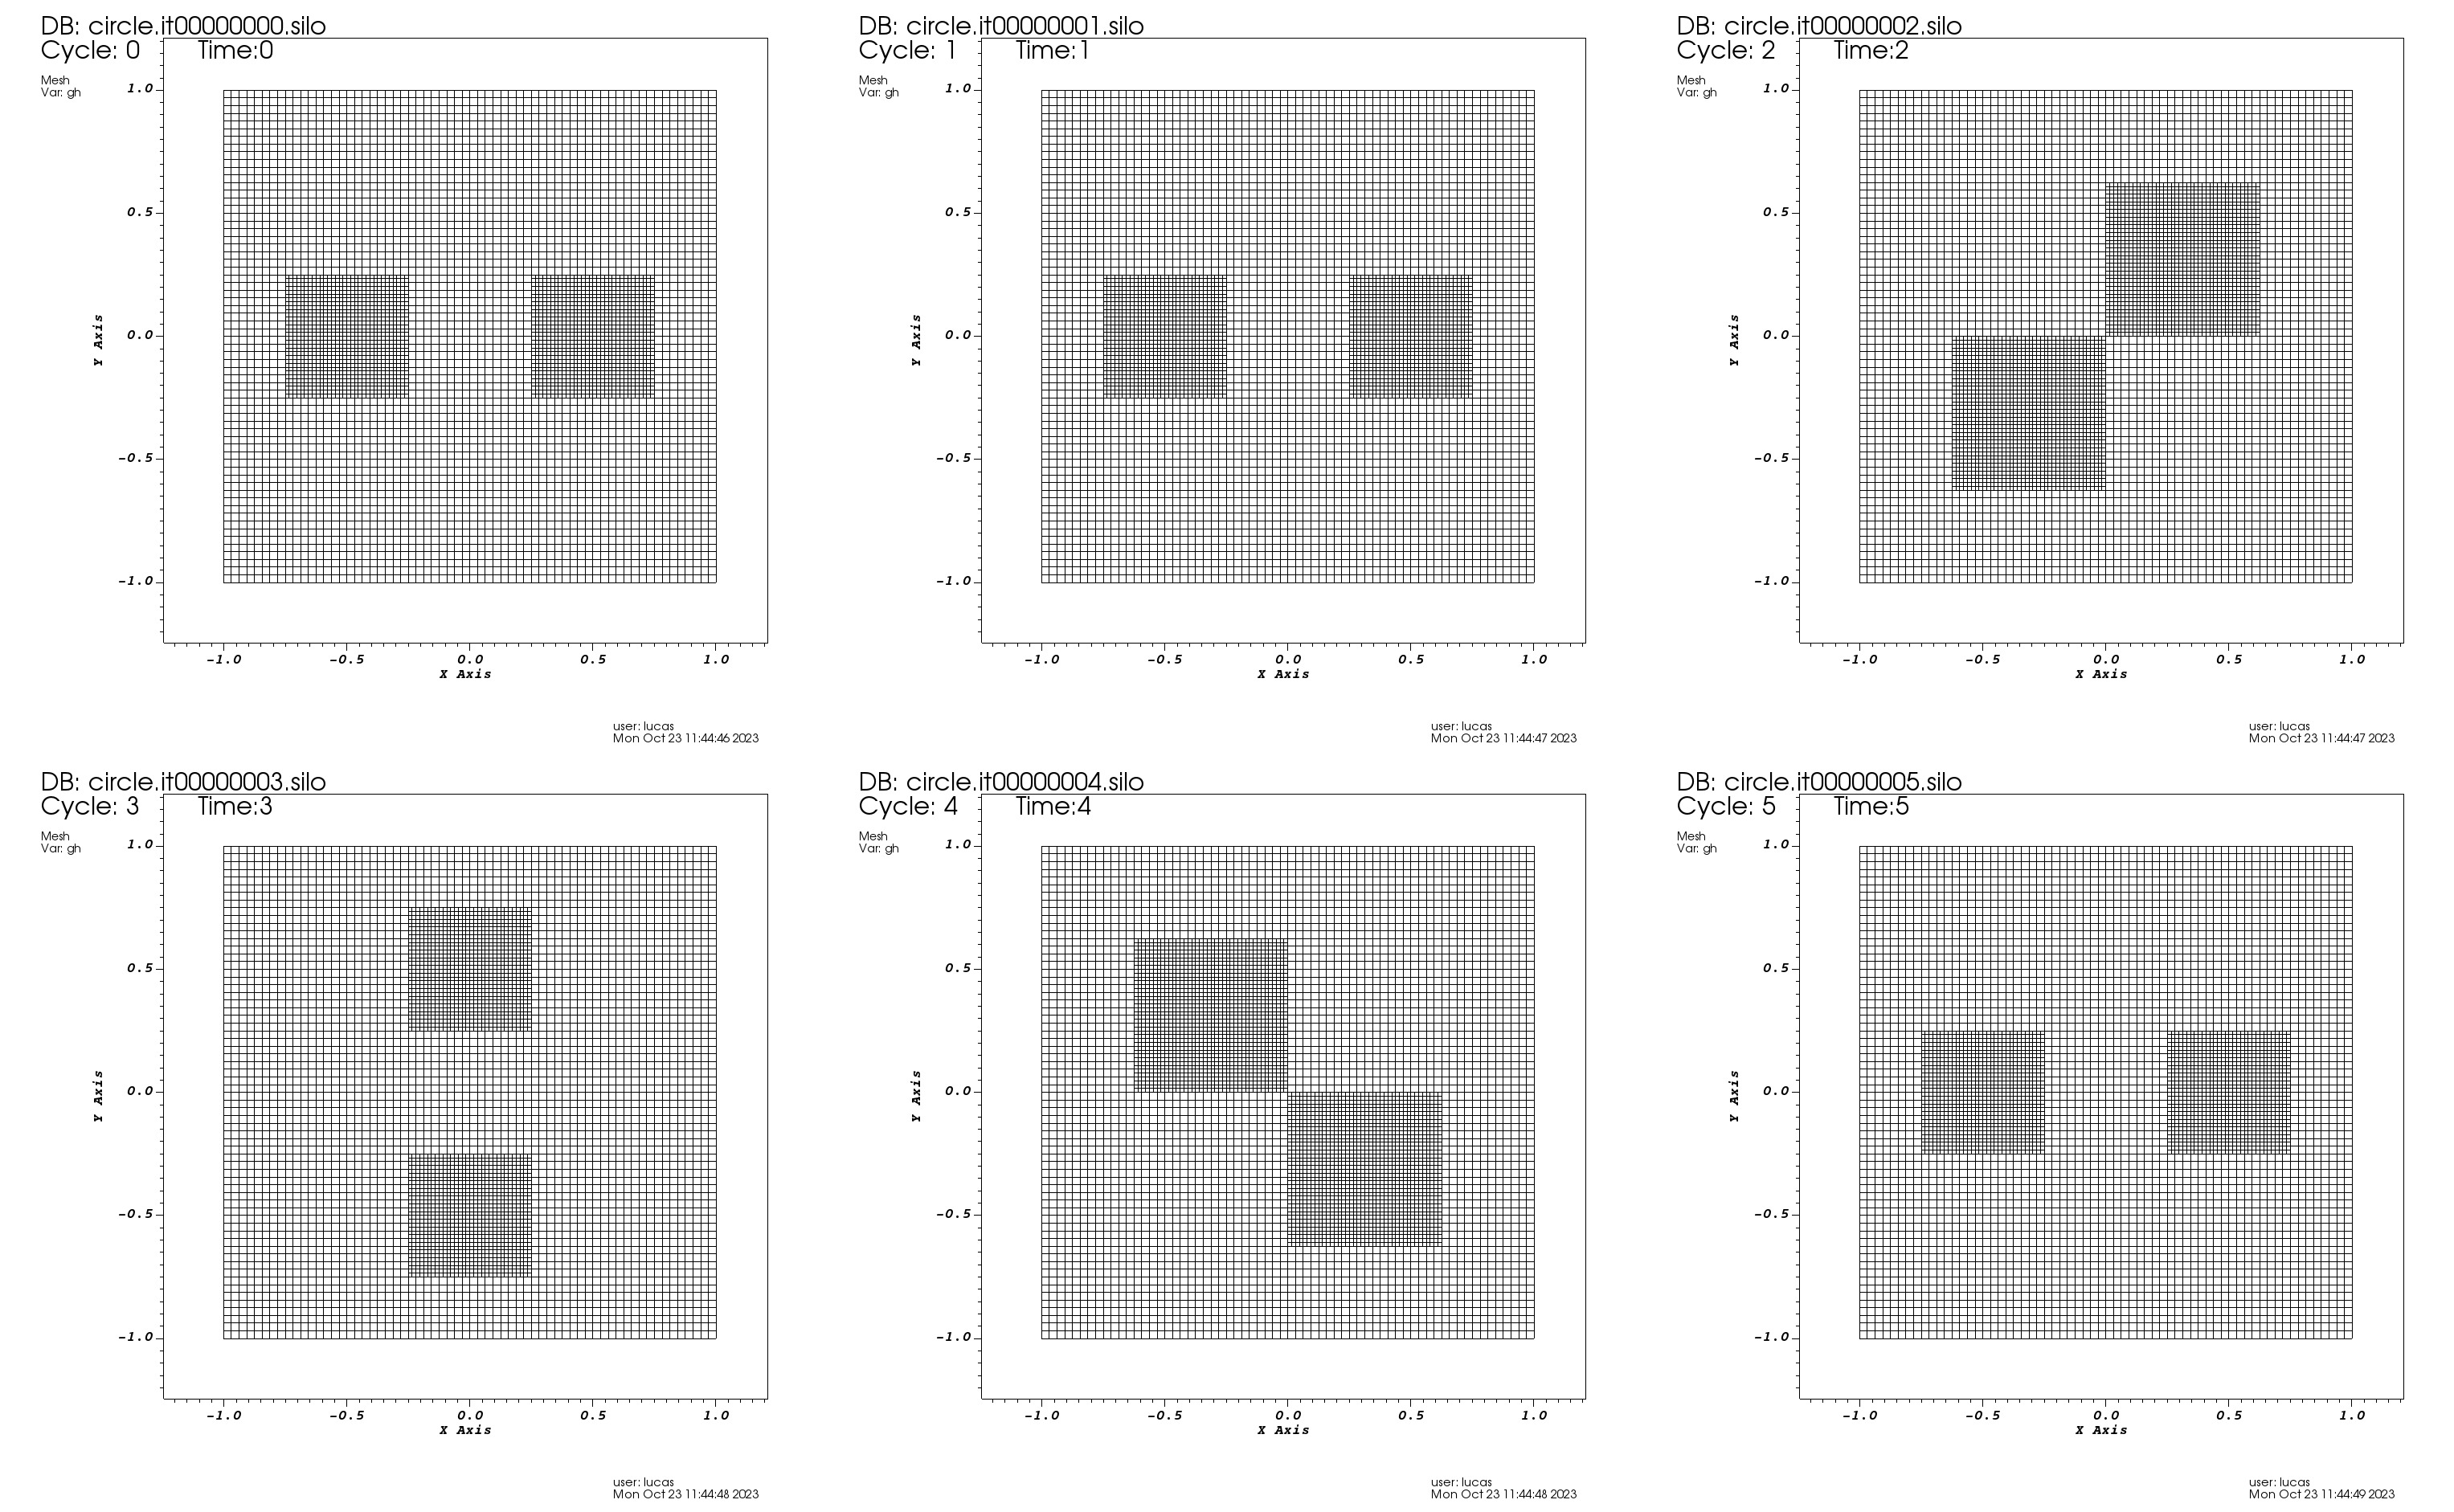
\includegraphics[width=\linewidth]{boxes_frames.png}
  \end{center}
  \caption{AMR boxes moving around a circle, as implemented in the \texttt{MovingBoxToy} thorn.}
  \label{fig:boxes_circle}
\end{figure*}

\subsection{Advanced AMR}
\label{sec:advanced_amr}

\CarpetX\space supports non-fixed (adaptive) mesh refinement. For cell level control of AMR, \CarpetX\space provides user with a cell centered and non-checkpointed grid function called \texttt{regrid\_error}. Users are responsible for filling this grid function with real value however they see fit. Once it is filled, the configuration parameter \texttt{CarpetX::regrid\_error\_threshold} controls regridding: If the values stored in \texttt{regrid\_error} are larger than what is set in \texttt{regrid\_error\_threshold}, the region gets refined. Additionally, the configuration parameter \texttt{CarpetX::regrid\_every} controls how many iterations should pass before checking if the error threshold has been exceeded. The parameter \texttt{CarpetX::max\_num\_levels} controls the maximum number of allowed refinement levels.

Note that \CarpetX\space \textbf{does not} provide a ``standardized'' regrid error routine. This is because refinement criteria are highly specific to the problem being solved via AMR, and thus there is no one size fits all error criteria. This might seem inconvenient, but ultimately it allows for users to have higher degrees of customization in their AMR codes. For demonstration purposes, we shall now provide a routine that estimates the regrinding error as \todo{what? Provide a good starter example}. This implementation could be used as a starting point for codes that wish to use different error criteria in their AMR grids.

\begin{lstlisting}
  extern "C" void EstimateError(CCTK_ARGUMENTS) {
  DECLARE_CCTK_ARGUMENTSX_EstimateError;
  DECLARE_CCTK_PARAMETERS;

  // The template indices indicate this a loop over cell centers
  // Remember that regrid_error is a cell centered grid function
  grid.loop_int_device<1, 1, 1>(
      grid.nghostzones,
      [=] (const Loop::PointDesc &p) {
        // TODO: Give a simple example
        regrid_error(p.I) = 0.0;
      });
}
\end{lstlisting}

Once defined, \texttt{EstimateError} should be scheduled in both the \texttt{postinitial} and \texttt{poststep} bins. The \texttt{poststep} bin gets called right after a new state vector has been calculated, and is thus the proper place to analyze it. The \texttt{postinitial} scheduling is also necessary for computing the initial refinement after initial conditions have been set up. A thorn making use of the \texttt{regrid\_error} AMR mechanism should then add the following to its \texttt{schedule.ccl} file:

\begin{lstlisting}[language=bash]
  SCHEDULE EstimateError AT postinitial
  {
    LANG: C
    READS: state(everywhere)
    WRITES: CarpetX::regrid_error(interior)
  } "Estimate error for regridding"
  
  SCHEDULE EstimateError AT poststep
  {
    LANG: C
    READS: state(everywhere)
    WRITES: CarpetX::regrid_error(interior)
  } "Estimate error for regridding"
\end{lstlisting}

\subsection{Controlling prolongation}

\begin{lstlisting}[language=bash]
  KEYWORD prolongation_type "Prolongation type"
{
  "interpolate" :: "interpolate between data points"
  "conservative" :: "interpolate cell averages, ensuring conservation"
  "ddf" :: "interpolate in vertex centred and conserve in cell centred directions"
  "ddf-eno" :: "interpolate in vertex centred and ENO-conserve in cell centred directions"
  "ddf-hermite" :: "Hermite-interpolate in vertex centred and conserve in cell centred directions"
  "natural" :: "interpolate in vertex centred and conserve in cell centred directions, using the same order"
  "poly-cons3lfb" :: "interpolate polynomially in vertex centred directions and conserve with 3rd order accuracy and a linear fallback in cell centred directions"
} "ddf"

CCTK_INT prolongation_order "Prolongation order"
{
  0:* :: ""
} 1

BOOLEAN do_restrict "Automatically restrict fine to coarse grid functions"
{
} yes



BOOLEAN restrict_during_sync "Restrict fine to coarse grid functions when syncing"
{
} yes
\end{lstlisting}

%%%%%%%%%%%%%%%%%%%%%%%%%%%%%%%%%%%%%%%%%%%%%%%%%%%%%%%%%%%%
\section{Boundary conditions and symmetries}
\label{sec:bcs}
\CarpetX\space provides a way of setting up standard boundary conditions and symmetry conditions (to be applied on grid boundaries) via parameter files. In this section, we will describe the available options.

\subsection{Boundary conditions}

Users can choose between the following boundary condition types:

\begin{enumerate}
    \texttt{"none"}\: Don't apply any boundary condition to the grid. This is the default value in all directions"
    \texttt{"dirichlet"}\: Dirichlet boundary conditions.
    \texttt{"linear extrapolation"}: Linearly extrapolate interior values to boundary values.
    \texttt{"neumann"}: Neumann boundary conditions.
    \texttt{"robin"}: Robin boundary conditions.
\end{enumerate}



%%%%%%%%%%%%%%%%%%%%%%%%%%%%%%%%%%%%%%%%%%%%%%%%%%%%%%%%%%%%
\section{Interpolation}
\label{sec:interpolation}

%%%%%%%%%%%%%%%%%%%%%%%%%%%%%%%%%%%%%%%%%%%%%%%%%%%%%%%%%%%%
\section{Performance tuning}
\label{sec:perf_tuning}
\subsection{Parallelism model}

When running on CPUs, \AMReX\space will divide the grid in boxes whose sizes are controlled by \texttt{blocking\_factor} and \texttt{max\_grid\_size} parameter families. These will be distributed over MPI ranks and each rank will subdivide the boxes on \textit{tiles} that get assigned to CPU threads. Tile sizes are controlled via the max\_tile\_size parameter family.

\todo{How does this work in GPUs?}

\subsection{Parallelism control parameters}

\CarpetX\space allows users to control \texttt{AMReX}'s underlying load balancing mechanism by exposing \texttt{AMReX} parameters to \texttt{Cactus} parameter files. We shall now describe these parameters and their functionality.

\subsubsection{\texttt{CarpetX::max\_grid\_size\_\{xyz\}}}

\AMReX\space will divide the domain in every direction so that each grid is no longer than \texttt{max\_grid\_size} in that direction. It defaults to 32 in each coordinate direction.

\subsubsection{\texttt{CarpetX::blocking\_factor\_\{xyz\}}}

Constrain grid creation so that each grid must be divisible by \texttt{blocking\_factor}. This implies that both the domain (at each level) and \texttt{max\_grid\_size} must be divisible by \texttt{blocking\_factor}, and that \texttt{blocking\_factor} must be either 1 or a power of 2. It defaults to 8 in every direction.

\subsubsection{\texttt{CarpetX::refine\_grid\_layout}}

If set to \texttt{"yes"} and the number of grids created is less than the number of processors ($N_\text{grids} < N_\text{procs}$), then grids will be further subdivided until $N_\text{grids} \geq N_\text{procs}$. If subdividing the grids to achieve $N_\text{grids} \geq N_\text{procs}$ would violate the \texttt{blocking\_factor} criterion then additional grids are not created and the number of grids will remain less than the number of processors. It defaults to \texttt{"yes"}

\subsubsection{\texttt{CarpetX::grid\_efficiency}}

Because mesh refinement in \AMReX is done per-cell (see sec.~\ref{sec:advanced_amr} for further details), a refinement region may be irregular. \AMReX\space can only deal with logically cubical grids, thus a refinement region will be replaced by a new grid consisting of coarse and finer boxes on the region. Due to this ``discretization'' of the refinement region, more cells will be refined than necessary. Refining too many points becomes obviously inefficient. Conversely, refining too few points is also non-ideal, as it leads to a grid structure consisting of many small boxes. ``Grid efficiency'' then refers to the ratio of the points that need to be refined over the points that actually are refined in the new grid structure. This steers AMReX's eagerness to combine smaller boxes into larger ones by refining more points. The default value for this parameter is $0.7$

\subsubsection{\texttt{CarpetX::max\_tile\_size\_\{xyz\}}}

Controls the maximum tile size in each direction. Its default values are $1024000$ in the \texttt{x} direction, $16$ in the \texttt{y} direction and $32$ in the \texttt{z} direction.

%%%%%%%%%%%%%%%%%%%%%%%%%%%%%%%%%%%%%%%%%%%%%%%%%%%%%%%%%%%%
\section{Profiling}
\label{sec:profiling}
Profiling refers to the act of collecting runtime and other performance data on the execution of an application in order to improve its performance characteristics. The recommended way of profiling \CarpetX\space applications is using \href{http://hpctoolkit.org/}{\texttt{HPCToolkit}}. We recommend that user first read the software's \href{http://hpctoolkit.org/manual/HPCToolkit-users-manual.pdf}{documentation} thoroughly. 

Installing \texttt{HPCToolkit} on an HPC system will probably require the help of the system's administrators. Once installed, the application should be launched with the \texttt{hpcrun} command, which will automatically collect performance data from the launched application. To profile \CarpetX\space while using an HPC system, the recommended steps are:
%
\begin{enumerate}
  \item Launch an interactive section with the cluster's job system. In this session, the \texttt{mpirun} and \texttt{hpcrun} commands should be available.
  
  \item Navigate to the directory where the \Cactus\space executable is located. Given a configuration named \texttt{config-name}, the executable is located in \texttt{Cactus/exe/cactus\_config-name}.
  
  \item Select a parameter file to execute and gather performance information on. Let us call it \texttt{perf.par} and suppose that it is located in \texttt{Cactus/exe/}.
  
  \item Assuming that the system's \texttt{MPI} launcher is called \texttt{mpirun}, to profile a CPU application, issue
  %
  \begin{lstlisting}[language=bash]
    mpirun hpcrun ./cactus_config-name perf.par
  \end{lstlisting}
  %
  To profile a GPU application, issue
  %
  \begin{lstlisting}[language=bash]
    mpirun hpcrun -e gpu=<vendor> ./cactus_config-name perf.par
  \end{lstlisting}
  %
  where \texttt{<vendor>} is either \texttt{nvidia} or \texttt{amd}, depending on which GPU chips are available in the system.

  \item After \Cactus\space completes the evolution, a new folder called \texttt{hpctoolkit-cactus\_config-name-measurements} will be created on the same directory where \texttt{hpcrun} was executed. \texttt{HPCToolkit} needs to recover program structure in order to create better profiling information. To do that, issue
  %
  \begin{lstlisting}[language=bash]
    hpcstruct hpctoolkit-cactus_config-name-measurements
  \end{lstlisting}

  \item Finally, to have \texttt{HPCToolkit} analyze measurements and attribute it to source code, issue
  %
  \begin{lstlisting}[language=bash]
    hpcprof hpctoolkit-cactus_config-name-measurements
  \end{lstlisting}
\end{enumerate}

This will generate the \texttt{hpctoolkit-cactus\_config-name-database} folder, which can be used with \texttt{HPCToolkit}'s provided profile visualization tool called \href{http://hpctoolkit.org/download.html}{\texttt{hpcviewer}}. See chapter 10 of the \texttt{HPCToolkit} \href{http://hpctoolkit.org/manual/HPCToolkit-users-manual.pdf}{manual} for usage details.

%%%%%%%%%%%%%%%%%%%%%%%%%%%%%%%%%%%%%%%%%%%%%%%%%%%%%%%%%%%%
\section{Outputting data}
\label{sec:data}
\subsection{SILO}
\label{sec:silo}

\subsection{OpenPMD}
\label{sec:openpmd}

\subsection{TSV}
\label{sec:tsv}

%%%%%%%%%%%%%%%%%%%%%%%%%%%%%%%%%%%%%%%%%%%%%%%%%%%%%%%%%%%%
\section{Debugging}
\label{sec:debugging}
To debug \CarpetX\space applications, users have access to the following parameters: 
%
\begin{itemize}
    \item \texttt{verbose}: A boolean parameter that controls weather or not \CarpetX\space produces verbose output. This output details more of what the driver is doing internally, aiding users in finding bugs. Its default value is \texttt{no}.

    \item \texttt{poison\_undefined\_values}: Sets undefined grid point values to \texttt{NaN} (not a number). By visualizing locations where grid functions contain \texttt{NaN}s, users can determine which grid points are not being filled correctly. Its default value is \texttt{yes}.
\end{itemize}

%%%%%%%%%%%%%%%%%%%%%%%%%%%%%%%%%%%%%%%%%%%%%%%%%%%%%%%%%%%%
\section{Acknowledgements}

\begin{thebibliography}{9}
\end{thebibliography}

% Do not delete next line
% END CACTUS THORNGUIDE

\end{document}
